\listfiles
\documentclass[manuscript, review, screen]{acmart}
%\setcitestyle{super,sort&compress}
\citestyle{acmauthoryear}
\usepackage{graphicx}
\usepackage{amsmath, amsthm, amssymb}
\usepackage{amsfonts}
\usepackage{tabularx}
\usepackage{multirow}
\usepackage{booktabs}
\usepackage[printonlyused]{acronym}
\usepackage{paralist}
\usepackage{enumitem}
\usepackage{subcaption} 
\usepackage[ruled]{algorithm2e}
%\usepackage{algorithmic}

\setlist{nolistsep}

\newacro{PGCE}{Postgraduate Certificate of Education}
\newacro{UTToF}{User Tracking Time-of-Flight}

\newcommand{\tickYes}{\checkmark}
\newcommand{\crossNo}{$\times$}

% Metadata Information
% \acmJournal{TOCHI}
% \acmVolume{9}
% \acmNumber{4}
% \acmArticle{39}
% \acmYear{2018}
% \acmMonth{3}

% Copyright
%\setcopyright{acmcopyright}
\setcopyright{acmlicensed}
%\setcopyright{rightsretained}
%\setcopyright{usgov}
%\setcopyright{usgovmixed}
%\setcopyright{cagov}
%\setcopyright{cagovmixed}

% DOI
\acmDOI{}

% Document starts
\begin{document}
% Title portion
\title{Controlling Classroom Technology with Upper-Body Gestures
  {\emph{and}} Improving Upper-Body Gesture Controls for Teacher Use}

\author{James McNaughton}
%\orcid{}
\affiliation{%
  \institution{Durham University}
  \streetaddress{South Road}
  \city{Durham}
  \postcode{DH1 3LE}
  \country{UK}}
\email{j.a.mcnaughton@durham.ac.uk}
\author{Tom Crick}
\orcid{0000-0001-5196-9389}
\affiliation{%
  \institution{Cardiff Metropolitan University}
  \streetaddress{Western Avenue}
  \city{Cardiff}
  \postcode{CF5 2YB}
  \country{UK}}
\email{tcrick@cardiffmet.ac.uk}


\renewcommand\shortauthors{McNaughton, J. and Crick, T.}

\begin{abstract}
{\emph{Abstract 1:}} There is a growing need to give teachers the ability to remotely control computer interfaces in the classroom.
Existing techniques such as control through fixed interfaces, mobile devices or voice commands have a number of short comings.
The use of upper-body gestures to allow teachers to control classroom interfaces as an alternative is considered.
For this alternative control technique a set of gestures which are intuitive to teachers must be identified.
Focus groups were used to discover which gestures are intuitively performed for specific actions relating to controlling classroom interfaces.
This paper details the gestures observed and details their implementation into a classroom control system.
The results of a controlled study using the implemented gesture system indicate that upper-body gesture controls are quicker than alternative technologies.
However, the use of the Kinect in the gesture system's current implementation yields too high of an error rate for the results to be conclusive.

{\emph{Abstract 2:}} As computers become more prevalent in classrooms, the need for systems which allow teachers to effectively control them increases.
An open-air gesture based control system using the Microsoft Kinect was created which allowed teachers to control instances of the SynergyNet framework in classrooms.
Despite the open-air gesture controls being quicker and less intrusive on teacher-student interaction than alternative technologies, its use was made unsuitable for use in the classroom due to issues relating to its accuracy and intuitiveness.
A number of changes were implemented into the system in an attempt to resolve these issues.
These changes were; the use of multiple Kinects, creation of a point-to-select gesture, improvements to the control sequence and the creation of a more cohesive gesture set.
A controlled study took place to evaluate whether these changes made the use of open-air gestures a viable method of controlling classroom technology.
Despite a significant improvement to system's intuitiveness, the Kinect's accuracy was still the cause of a number of problems.
With the use of a more accurate sensing technology the system would be suitable for controlling classroom technologies.
%\\
%\\ 
% \textbf{RESEARCH HIGHLIGHTS:}\\
% \textbullet \ A framework for assessing upper-body gestures is presented. \ 
% \textbullet \ A list of gestures suited for use with the Kinect in a classroom is produced.  \ 
% \textbullet \ A system which uses the Kinect to allow teachers to control classroom technology is implemented.  \ 
% \textbullet \ Issues with the Kinect device and gesture set are shown to be problematic.
\end{abstract}


%
% The code below should be generated by the tool at
% http://dl.acm.org/ccs.cfm
% Please copy and paste the code instead of the example below.
%


%
% End generated code
%

\keywords{Kinect, gestures, education, classroom technology, control}

\maketitle

%-------------------------------------------------------------------------

\section{Introduction}
\label{sec:intro}

The uses of technology in the classroom are growing~\cite{Lloyd2011,Robertson2012,Schrum2008}.
With this growth, the need for teachers to be able to control the deployed technologies increases~\cite{Apple1990,Selwyn2010,Selwyn2011}.
Without the ability to influence or control classroom technology, teachers may be unable to manage learning interaction or intervene when students start to lose focus on their current task~\cite{Chen2005,Karabenick2011}.

% With technology becoming more prevalent in the classroom~\cite{Lloyd2011,Robertson2012,Schrum2008} the likelihood of there being a number of student-orientated interfaces present in the environment increases.
% Due to the student-orientated nature of these interfaces teachers may have difficulty in attaining students' attention or assisting them with tasks~\cite{Chen2005,Karabenick2011}.
% This is because control of these interfaces lies primarily in the hands of the student.
% There is therefore a need for teachers to have some degree of control over these interfaces~\cite{Apple1990,Selwyn2010,Selwyn2011}.

Many current systems that allow teachers to control technology in the classroom require the use of a teacher-centric interface~\cite{Dagdag2011,Kuhn2005,Vila,Zhou2010}.
Whether static, where the interface remains stationary during its use, or mobile, where the interface can be carried to new locations during its use, these interfaces require the teacher to momentarily take their attention away from the students.
This division of attention caused by the distraction of an interface could have a detrimental effect on the quality of a teacher's interaction with their students.
The disruption in communication between the students and the teacher this causes can be undesirable in many circumstances.
Therefore, a method of controlling technology in the classroom without breaking this interaction would be beneficial.
One such possible method is to make use of physical gestures, where a user performs an action which is identified by a monitoring system, to issue commands to technology in the classroom.

The use of gestures, rather than a more standard interface, could allow teachers to issue commands in a more effective manner.
Time is saved by not requiring the teacher to travel to their control interface.
Even when there is no travel time, such as when mobile interfaces are used, gestures have the potential to be executed quicker than alternative input and control methods~\cite{Dulberg1999,Moyle2001}.
Quicker execution of the commands should afford the teacher more time to observe and aid students.
In addition, physical gestures should be less intrusive on the interaction between students and the teacher. 
Many interfaces, specifically touch-screen mobile devices such as tablets, do not facilitate eyes-free interaction~\cite{Brewster2003}.
This means that teachers using a static or mobile interface which utilises a visual output are required to dedicate a portion of their attention to its use.
This division of attention can interrupt interaction between teachers and students.
The use of physical gestures should allow teachers to continue interacting with students while issuing commands to a classroom technology's control system.

Teachers in technology enhanced classroom also acquire additional administration responsibilities~\citep{Kuhn2005} such as managing the consequence of faults with the devices used.
A physical gesture interface may reduce the overheads of such additional responsibilities by allowing teachers to quickly execute administrative tasks from any location in the classroom.

The potential benefits of physical gestures make its implementation into a classroom software framework desirable.
For a system such as this, a series of gestures must be produced which can be used to execute the various control commands within the framework.

% This paper focuses on SynergyNet~\cite{HatchA.HigginsS&Mercier2009}, a multi-touch framework intended for use in the classroom.
% The framework is built to support applications designed to be used by students through multi-touch interfaces.
% The SynergyNet lab, built around the framework's use, consists of a number of multi-touch tabletop surfaces and is arranged to resemble a classroom.
% The SynergyNet framework allows interaction between the multi-touch interfaces which enables the sharing of materials and the ability to issue commands through a network.
% The ability for commands to be sent across a network offers the opportunity for control to be remotely exerted over the tabletop interfaces.
% The SynergyNet framework has been augmented to use upper-body gestures, a subset of open-air gestures, to allow teachers to control classroom interfaces.
% However, previous studies have identified issues that make its use in the classroom unsuitable~\cite{McNaughton2013a}.

% The gesture controls enable the orchestration of several common-place commands, such as sending or retrieving materials.
% It is through that issues relating to the SynergyNet framework's upper-body gesture support may be present in similar open-air gesture driven systems.
% Therefore, any improvements which resolve the issues observed in the SynergyNet framework could be employed in other gesture systems. 
% These improvements have the potential to benefit any systems with similar technologies, control sequences or gesture sets.

The remainder of this paper is as follows. 
Section~\ref{sec:related} discusses gesture detection technologies, specifically time-of-flight cameras.
Section~\ref{sec:classcontrol} considers how the time-of-flight cameras could be used to adapt a classroom-based technology to utilise physical gestures.
What constitutes an effective gesture is discussed in Section~\ref{sec:gestures}.
A focus group based study is outlined in Section~\ref{sec:focusgroup} which was carried out to identify intuitive gestures for classroom control commands.
The results of the study are outlined in Section~\ref{sec:focusgroupresults} and their implications are discussed in Section~\ref{sec:discussion}. 
Implementation of a user generated set of gestures from observations on the focus group is detailed in Section~\ref{sec:implementation}.
Section~\ref{sec:evaluation} discusses a study using the implemented physical gesture control system.
Section~\ref{sec:evaluationresults} presents the results of this study and Section~\ref{sec:evaluationdiscussion} elaborates on the implications of the results.
Future developments utilising findings from the study and our conclusions are presented in Section~\ref{sec:conclusions}.

% The remainder of this paper is as follows. 
% Section~\ref{sec:related} discusses the existing control systems used in SynergyNet for issuing commands and current developments in using the Kinect to track open-air gestures.
% SynergyNet's support for upper-body gestures is discussed in detail in Section~\ref{sec:gestures}.
% The issues observed in SynergyNet's current gesture control system are outlined in Section~\ref{sec:issues}.
% Potential solutions used in other works to resolve these issues are discussed Section~\ref{sec:improvements}.
% Section~\ref{sec:implementation} details how improvements were implemented into the SynergyNet framework to resolve these issues.
% A user study is then outlined in Section~\ref{sec:study} which was carried out to assess the improved gesture system alongside the existing control technologies.
% The results of the study are outlined in Section~\ref{sec:results} and their implications are discussed in Section~\ref{sec:discussion}.
% Future developments utilising findings from the study and our conclusions are presented in Section~\ref{sec:conclusion}.

%-------------------------------------------------------------------------

\section{Background} 
\label{sec:related}

To allow a system to identify physical gestures a method of tracking the movements of users is required.
Time-of-flight cameras~\cite{Lange2001} are capable of doing this through building a depth image of an environment and tracking movement by identifying areas where the depth values change.
The Canesta~\cite{Yang2007} and 3DV~\cite{Wilson2007a} devices are both examples of these cameras.
The devices emit beams of infra-red light which can then be seen through an infra-red camera.
Using knowledge of the infra-red light emitted, the devices can identify where the beams are interrupted by an object.
This positional information allows the devices to build a depth image of an environment.
Thus, devices can identify the distance between itself and any item within the range of its infra-red beams.
However, both the Canesta~\cite{Yang2007} and 3DV~\cite{Wilson2007a} devices provide a low quality depth image.
There are alternatives which provide much more detailed depth images, such as Oblong's Mezzanine~\cite{kramer2011}.
However, the cost of the alternatives can also be prohibitive.
Devices which occupy the middle-ground between quality depth images and cost are also available.
Such devices include the Microsoft Kinect, shown in Figure~\ref{fig:kinect} and the Primesense sensor~\cite{Wilson2010}.
These devices are accurate enough to track user movement and have previously been used as part of gesture monitoring systems~\cite{Goth2011}.

\begin{figure}[h]
   \centering
   \includegraphics[width=0.45\textwidth]{figures/kinect.png}
   \caption{The Microsoft Kinect.}
   \label{fig:kinect}
\end{figure}

The firmware of \ac{UTToF} cameras, like the Kinect and Primesense sensor, offer several features relating to the tracking of a user.
These devices can outline any persons in front of the device and differentiate between them using their distances from the camera.
The device can then identify and give positional information on specific parts of a person's body, such as their limbs and joints if a calibration technique is executed.
This is usually a pose assumed by a person which allows the device to view a specific human outline from which it can identify joints and limbs~\cite{Xia2011}.
Using the difference between frames from the depth camera, the device's firmware can track the movement of people in its field of view.

The information a \ac{UTToF} camera can give concerning the positions of a person and their limbs offers a wealth of possibilities regarding computer interaction.
Specifically, the ability to obtain the positional information of people may be of use for co-located interfaces where interaction may require knowledge of the position of the user.
The ability to track and differentiate between users comes in useful for interaction technologies which allow users to share interfaces.
Dietz and Leigh~\cite{Dietz2001} note how the ability to track a user can be important.
Their research also identifies how existing techniques for tracking user positions which entail encumbering the user with extra devices are undesirable.
\ac{UTToF} cameras offer the opportunity to track people without the need for users to wear additional devices.

\ac{UTToF} cameras allow users to move about an environment without being constrained to an interface.
This is beneficial for teachers in classroom environment for whom mobility is vital.
There are alternatives to physical gesture sensing technologies, like \ac{UTToF} cameras, which also afford this type of freedom from the interface.
Voice control is one such alternative where the teacher could issue commands to a technological framework in the classroom through a series of spoken instructions.
Using physical gestures alongside the voice commands could be beneficial as shown in the work of Bolt~\citeyearpar{Bolt1980}.
Allowing the user to gesture at where they want a specific command to influence reduces the need for additional spoken instructions.
However, the ambient noise in a typical classroom is likely to be too loud for voice recognition technologies~\cite{Cavalier1996,Goette1998,OHare1999}.
In addition to this caveat, the issuing of voice commands also will require teachers to interrupt their conversations with their students.

The use of physical gestures monitored via a \ac{UTToF} camera appears to be the most suitable approach to creating a system which allows teachers to control classroom technologies without the requirement for a distracting interface.

%-------------------------------------------------------------------------

% \section{Background} 
% \label{sec:related}

% %\begin{figure}[h]
% %   \centering
% %   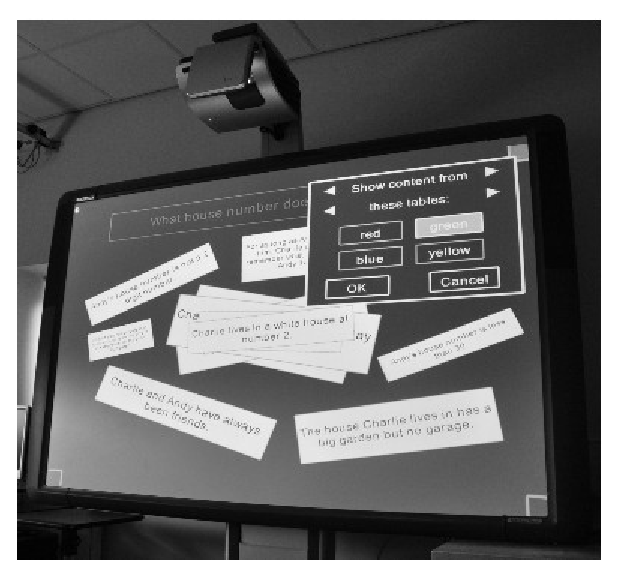
\includegraphics[width=0.45\textwidth]{fig1.eps}
% %   \caption{The multi-touch board used to control SynergyNet.}
% %   \label{fig:controlBoard}
% %\end{figure}

% SynergyNet supports numerous control technologies which teachers can use to control instances of the framework on student-centric multi-touch interfaces.
% The first of these supported technologies is a multi-touch interface.
% The teacher controls used for this technology are implemented as a typical SynergyNet application.
% This allows the teacher to use any multi-touch device capable of running the framework to control the environment's student-centric interfaces.
% This set of teacher controls has been made available to teachers in the SynergyNet lab through one of two multi-touch devices; a board and a podium.

% The multi-touch board used in the SynergyNet lab for issuing commands to the students' interfaces is shown in Figure~\ref{fig:controlBoard} running an instance of the teacher controls.
% Both the podium and board devices are static.
% Due to this the teacher is required to be positioned in close proximity to them in order to issue any control commands.
% This requirement of the devices can be detrimental on interaction between the teacher and students.
% This is because whenever the teacher wishes to issue a control command they will be required move away from the students to one of the devices.
% The time taken to travel to the device can prolong the break in interaction between the students and the teacher.

% %\begin{figure}[h]
% %   \centering
% %   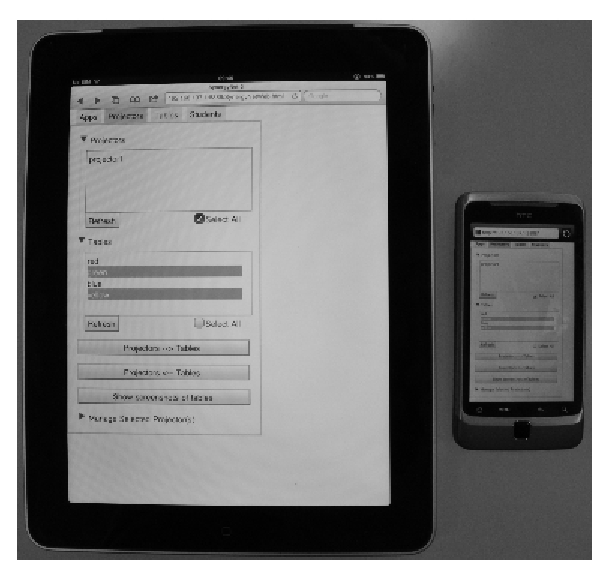
\includegraphics[width=0.45\textwidth]{fig2.eps}
% %   \caption{The web interface which controls SynergyNet accessed through a tablet device.}
% %   \label{fig:controlTablet}
% %\end{figure}

% To resolve the potential problem of breaking interaction with students to issue commands through static interfaces, controls which can be accessed through a range of mobile devices were implemented into SynergyNet.
% These controls, shown in Figure~\ref{fig:controlTablet}, are built to be accessed through any device capable of joining a wireless network and displaying web-based content.
% The controls can be accessed by teachers through devices such as smart-phones and tablets.
% Despite the mobile nature of these interfaces, they have been noted in previous studies~\cite{Hatch2011} to remove the teacher's attention from the students.
% Teachers were also noted to take a significant amount of time to issue commands through the mobile interface, prolonging the break in interaction with the students.
% The interaction between students and teachers is required to ensure that students stay on task and that teachers are able to monitor the student's performance \cite{Hall1968}.
% This break in interaction can be detrimental for both a student's ability to learn and the teacher's ability to maintain order in the classroom \cite{Shirley2010}.
% A system of control which allows teachers to quickly issue commands without interrupting their interaction with their students would be beneficial.

% Utilising open-air gestures could allow teachers to issue commands without the requirement to concentrate on an interface~\cite{Varona2009,Wachs2011}.
% The term \lq open-air gesture\rq\ is used to refer to gestures performed by users which do not require contact with an interface.

% %\begin{figure}[h]
% %   \centering
% %   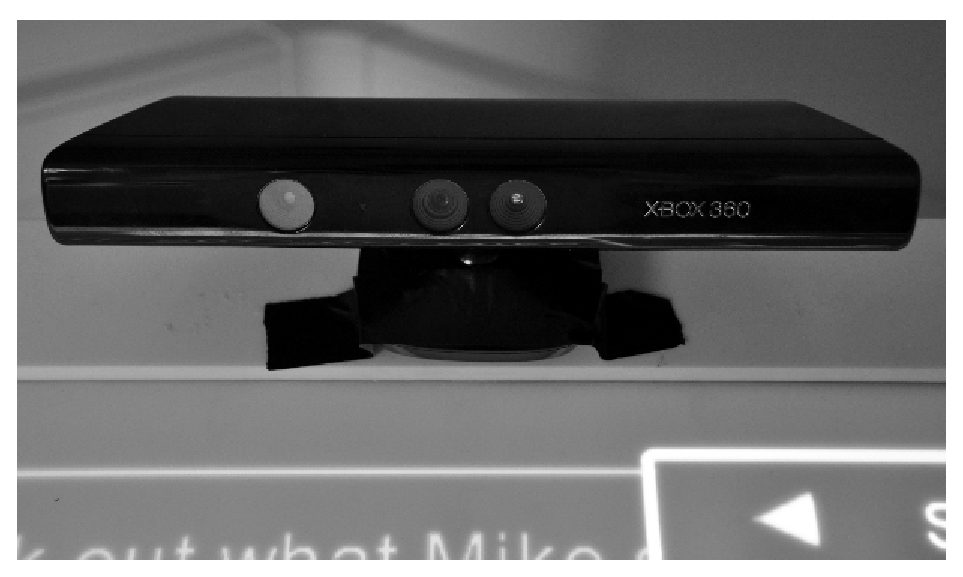
\includegraphics[width=0.45\textwidth]{fig3.eps}
% %   \caption{Microsoft's Kinect.}
% %   \label{fig:controlKinect}
% %\end{figure}

% The Microsoft Kinect, shown in Figure~\ref{fig:controlKinect}, can be used to support the detection of open-air gestures~\cite{Goth2011}.
% The Kinect is a low-cost device which is capable of capturing both RGB and depth information about an environment.
% The RGB data is captured through a typical visible light camera and the depth data through an infra-red camera. 
% The device projects an infra-red light pattern which the Kinect can see and identify.
% The Kinect can then use deformations of the pattern it views to identify surfaces and their distances from the device.
% This method of depth-sensing is known as a structured light pattern~\cite{Salvi2010}.
% Using both RGB and depth data the Kinect is capable of tracking persons about an environment.
% Once a person performs a calibration gesture, the Kinect is then capable of tracking that person's limbs and joints.

% Being able to track the location of a person's limbs and joints allows for a system to be built around the Kinect's output which can identify gestures performed by a user~\cite{Davison2012,Lai2012,Patsadu2012}.
% Once calibrated, a teacher could perform gestures which, when identified by the recognition system, would trigger the sending of commands to student-centric interfaces.
%-------------------------------------------------------------------------

\section{Classroom Control with Gestures}  
\label{sec:classcontrol}

The ability to track specific users and their limbs allows a \ac{UTToF} camera to be used for identifying body-orientated gestures.
This could allow teachers to control technology in the classroom without the need for an intermediate physical interface.
Teachers would not be encumbered with a device allowing them freedom to move about the classroom.
Since physical gestures would permit eyes-free interaction~\citep{Brewster2003} with a control system, teachers could interact with students without losing control of the technology.
Due to a \ac{UTToF} camera's ability to track people in an environment, once a teacher is identified their movement around the classroom can be followed.
As a result of this, teachers could potentially issue commands through gestures anywhere in the classroom.

\ac{UTToF} cameras have high availability and relatively low cost in comparison to alternative depth sensing devices such as those used in Oblong's Mezzanine~\citep{kramer2011}.
Despite these potential benefits of \ac{UTToF} camera, there are several limitations that must be considered.
One limitation is their accuracy.
\ac{UTToF} cameras are capable of tracking users and the position of their limbs.
However, for a \ac{UTToF} camera to track anything more precise, such as fingers, additional constraints on their abilities will need to be imposed \citep{Clark2011}.
These additional limitations potentially include a reduction in range, a reduced limit on the number of tracked users and the use of encumbering devices.
All these limitations are undesirable for the use of the device in the classroom.
Therefore, in the work discussed here, \ac{UTToF} camera will be assumed not be augmented to track anything more precise than user limbs.
This means that any gestures to be used by teachers for issuing control commands should consist of limb positioning and movement.

\begin{figure}[t]
   \centering
   \includegraphics[width=0.45\textwidth]{figures/gestures_venn_diagram.png}
   \caption{The hierarchy and intersection of physical gesture sets.}
   \label{fig:gestureVenn}
\end{figure}

Figure~\ref{fig:gestureVenn} represents the different sub-sets of physical gestures.
The inability of an un-augmented \ac{UTToF} camera to track anything more precise than user limbs discounts the adoption of gesture sets 4 and 5, i.e. gestures which use fingers, for use in the classroom.
Any gesture which lies outside the grouping of those which can be identified by a \ac{UTToF} camera must be discounted.
This results in gestures sets 1, 2 and 3 also being deemed unsuitable for classroom use.

There are several reasons for gestures involving the use of the lower body limbs and joints, such as the legs, to be discounted.
One such reason is their requirement for the visibility of the lower body.
In a classroom full of furniture and seated students, the teacher's lower body will potentially be obscured most of the time from the view of the \ac{UTToF} camera.
The requirement for a teacher to move to a position where their lower body is visible to the \ac{UTToF} camera counters the device's potential benefit of allowing for control of the system without the need to move away from students.

Another reason for discounting gestures using lower limbs and joints is that the movement of the teacher's legs may affect their balance which could result in accidents.
In addition to this, gestures utilising a teacher's legs may require the teacher to be standing when performing them.
This could interrupt interaction with students if the teacher is seated while in discussion with them.
Gestures which do not require teachers to stand would allow the teacher to issue commands while still being seated.
Due to these reasons, only gestures which utilise the positioning and movement of the upper-body should be considered when developing a classroom control system.
This means that gestures should only make use of upper-body joints and limbs which a \ac{UTToF} camera can track: the torso, wrists, hands, elbows, shoulders, neck and head.
Therefore, gesture sets 6 and 7 in Figure~\ref{fig:gestureVenn} are shown to be unsuitable for use in the classroom.

% \begin{table}[h]
% \processtable{Unique physical gesture sets.\label{table:gestures}}{
% \begin{tabular}{!{\vrule width 1.5pt}c|c|c|c|c!{\vrule width 1.5pt}}
% \noalign{\hrule height 1.5pt}
% \textbf{} 			&\textbf{Uses}	&\textbf{Uses}	&\textbf{} 	&\textbf{Visible to}	\\
% \textbf{Gesture} 	&\textbf{Upper-}	&\textbf{Lower-}	&\textbf{Uses} 	&\textbf{a \ac{UTToF}}	\\
% \textbf{Set} 		&\textbf{body} 	&\textbf{body} 	&\textbf{Fingers}	&\textbf{camera}			\\
% \cline{1-5}
% 1			&\tickYes 				&\crossNo			&\crossNo				&\crossNo			\\
% \cline{1-5}
% 2			& \crossNo				&\tickYes 			&\crossNo				&\crossNo			\\
% \cline{1-5}
% 3			&\tickYes  				&\tickYes 			&\crossNo				&\crossNo			\\
% \cline{1-5}
% 4			&\tickYes  				&\crossNo 			&\tickYes 				&\crossNo			\\
% \cline{1-5}
% 5			&\tickYes  				&\tickYes 			&\tickYes 				&\crossNo			\\
% \cline{1-5}
% 6			&\crossNo 				&\tickYes 			&\crossNo				&\tickYes 			\\
% \cline{1-5}
% 7			&\tickYes  				&\tickYes 			&\crossNo				&\tickYes 			\\
% \noalign{\hrule height 1.5pt}
% 8 			&\tickYes  				&\crossNo 			&\crossNo				&\tickYes 			\\
% \noalign{\hrule height 1.5pt}
% \end{tabular}}{}
% \end{table}


As Table~\ref{table:gestures} shows, only gesture set 8 is suitable for use by a teacher in a classroom environment.
All other gesture sets have been discounted due to their use of lower body limbs or inability to be identified by a \ac{UTToF} camera.
Gesture set 8 consists of gestures which can be observed by a \ac{UTToF} camera that use the upper-body but not the lower-body or fingers.

\subsection{Potential Issues}  
\label{sec:attention}

The use of physical gestures in the classroom requires that several potential issues are accommodated for in the design of any system which supports them.

\subsubsection{False Positives}  
\label{sec:attention}

A potential issue concerning \ac{UTToF} cameras are that, by default, they are active at all times.
This means that teachers will need to be mindful of their actions.
Expressive body language or movement around the classroom could be interpreted by a \ac{UTToF} camera as a gesture.
This may trigger unwanted responses from any system utilising the device.
Therefore, a method of dismissing a \ac{UTToF} camera's attention and recapturing it later would be beneficial 
One potential solution to these false positives is to have designated areas from which gestures should be made.
This would allow teachers to move outside these areas without the possibility of accidentally issuing a command.
However, this solution does restrict the locations where the commands can be issues from, diminishing the ability of teachers to issue commands from anywhere.

A gesture based method of toggling a \ac{UTToF} camera's attention is another potential solution to the issue of a teacher unintentionally issuing commands through their movement in the classroom.
The \ac{UTToF} camera will not be able to issue any commands to a classroom technology unless its attention has been obtained by the teacher.
This results in the \ac{UTToF} camera used having two states: attentive and inattentive.
A gesture could be setup to be identified by the \ac{UTToF} camera in both states.
This gesture can be used to toggle state.
This diminishes the range of possible false gestures to one.
The solution reduces the chances of a teacher unintentionally issuing commands and allows for control over the \ac{UTToF} camera anywhere in the environment.
If this solution is adopted it is important to identify the gesture for gaining and dismissing the \ac{UTToF} camera's attention.

A potential drawback with the attention-toggling approach of managing these false positives is that if a teacher intentionally performs a gesture without getting the device's attention they will be ignored.
A false negative is preferable to a false positive because an unintended gesture may have irrecoverable consequences.
A false positive will have no consequence other than requiring the teacher to repeat their gesture again with the attention of the \ac{UTToF} camera.
Despite not being as problematic as the potential consequences of a false positive, the time-wasting result of a false negative is a potential issue.
A method of ensuring that a teacher knows whether they have the \ac{UTToF} camera's attention would be beneficial in stopping false negatives if the attention-toggling approach is taken.
Audible or visual feedback would aid the teacher in knowing whether their movement can or cannot be interpreted by the system as a gesture.

\subsubsection{Interface Selection}  
\label{sec:selection}

It is important to note that sometimes a teacher may not want to affect all interfaces when issuing a command.
This means that the teacher should be able to perform a gesture in such a way that the system is informed that the related action is intended to only affect specific interfaces.
A \ac{UTToF} camera's ability to track users can allow for the system to be informed of the location of a teacher in relation to the interfaces in the classroom.
Therefore, the teacher's proximity to interfaces could be used by a system to identify which devices a command should affect if informed of their locations.
However, the drawback to this approach is that if the teacher wishes to influence multiple interfaces they will be required to repeat the gesture in close proximity to each of the target interface.
This requires the teacher to move about the classroom and may interrupt their interactions with the students.
Therefore, an alternative method of identifying which gestures should be affected by a command is desirable.

%-------------------------------------------------------------------------

% \section{SynergyNet and Upper-body Gesture Controls}  
% \label{sec:gestures}

% %\begin{figure*}[t]
% %   \centering
% %   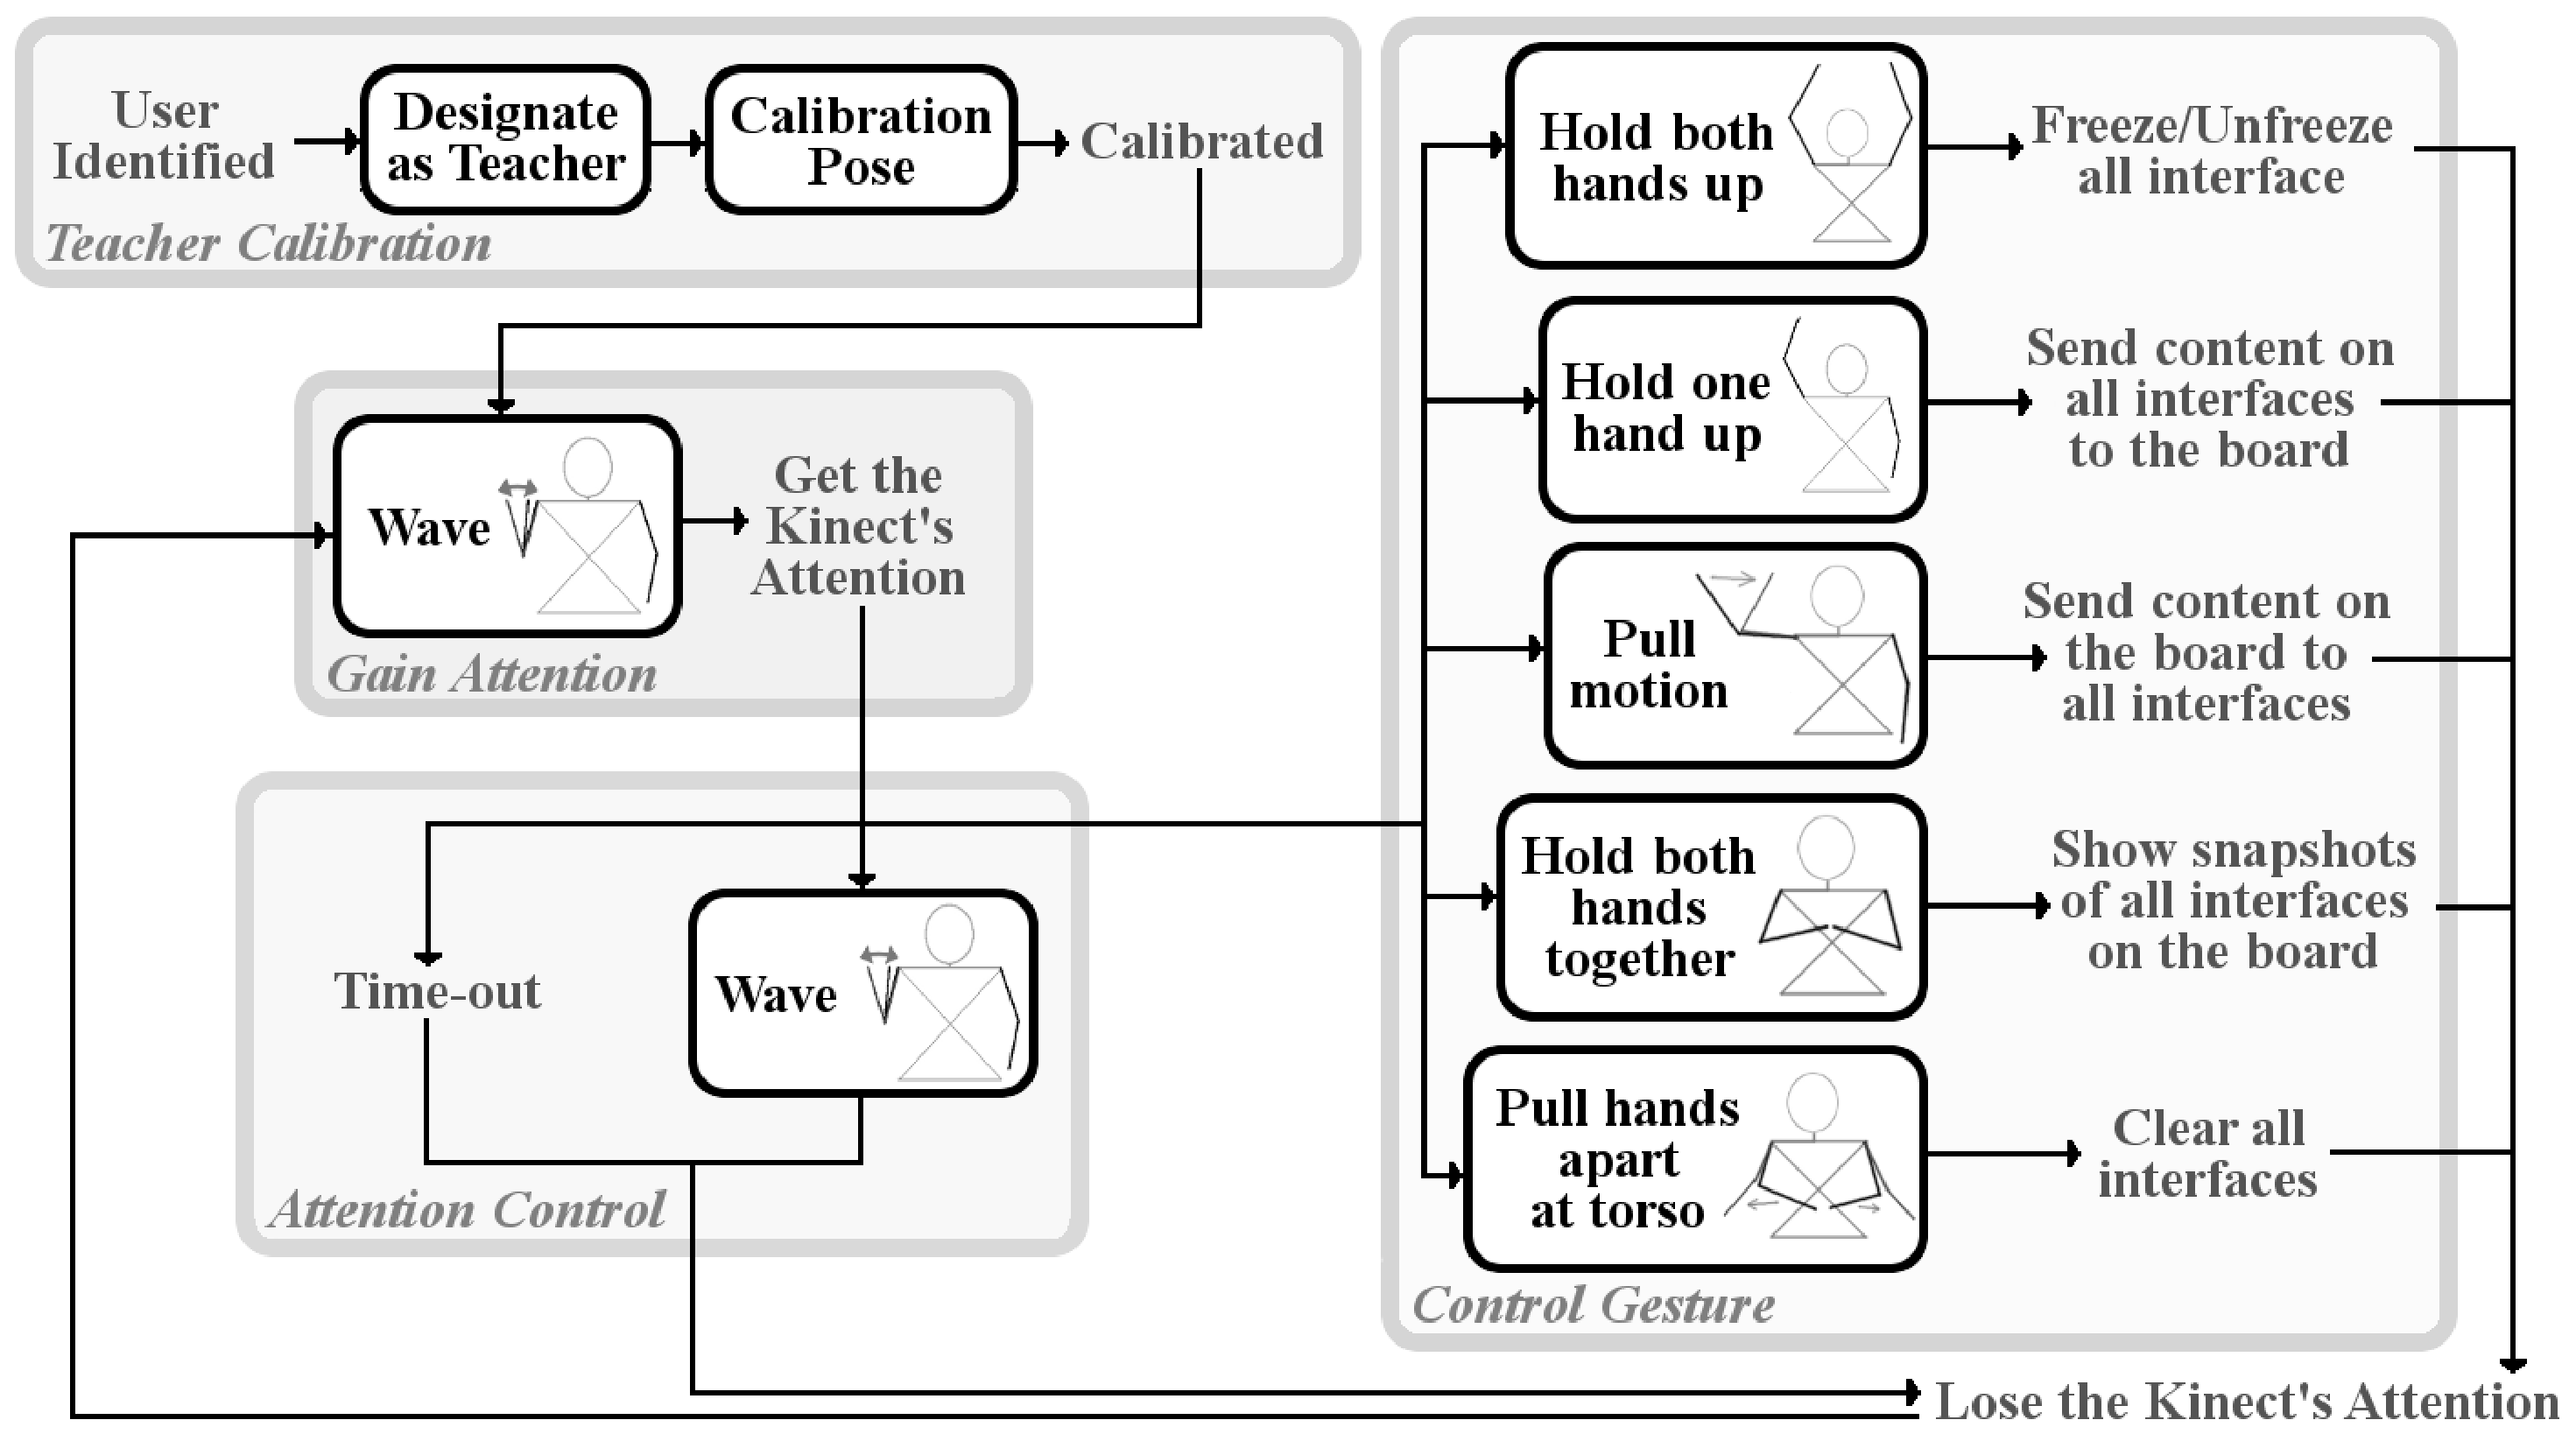
\includegraphics[width=1\textwidth]{fig4.eps}
% %   \caption{The existing control sequence implemented for the gesture controls in SynergyNet.}
% %   \label{fig:controlSequenceFlowDiagramOriginal}
% %\end{figure*}

% Using a set of gestures collated from a guessability study, a system for recognising gestures performed by a teacher was implemented into SynergyNet~\cite{McNaughton2013a}.
% This system can be used to issue specific commands to instances of the SynergyNet framework running on student-centric interfaces.

% The use of upper-body gestures to be used by SynergyNet was limited to those which could be performed with the joints and limbs of the upper-body.
% This includes the; torso, wrists, hands, elbows, shoulders, neck and head.
% The gestures do not include those which make use of the positioning or movement of fingers due to the loss of responsiveness required to support accurate finger tracking by the Kinect over large distances~\cite{Oikonomidis2011a,Oikonomidis2011b}.
% The issue of students and classroom furniture obscuring lower-body limbs and joints from the sensing device's view also led to the decision to exclusively use upper-body gestures.

% SynergyNet displays the current depth image collated by the Kinect as part of a GUI separate to any of the control systems.
% In this depth image identified persons are highlighted and labelled with the identification number allocated to them by the Kinect.
% Using these identifiers teachers can use the depth image to see discover the allocated number related to themselves.
% Through the GUI, teacher status can be granted to identified users with specific identification numbers.
% This allows the Kinect to be informed of which persons in the room are teachers.
% The Kinect will only look for gestures from persons who have been given a teacher status.

% Once a teacher is calibrated the Kinect can identify gestures through comparing the locations of limbs in relation to each other and their movement over time.
% Several of the gestures used by the SynergyNet framework are simple poses where a teacher will hold a specific limb or joint in position for a length of time.
% The remainder of the gestures used by the framework are defined by sequences of poses.

% Figure~\ref{fig:controlSequenceFlowDiagramOriginal} demonstrates the control sequence implemented into SynergyNet through which teachers can issue commands to instances of the framework.
% To avoid the possibility of teachers performing gestures when they don't intend to, a method of gaining and dismissing the attention of the Kinect through a waving gesture was implemented.
% After gaining the Kinect's attention, the teacher then has a choice.
% They can choose to dismiss the device's attention through waving if they wish to do nothing.
% This option is likely to be used when a teacher accidentally performs a wave gesture and acquires the Kinect's attention by mistake.
% Otherwise the teacher can then perform a command gesture.
% If a teacher does this, the corresponding command will be applied to all student-centric interfaces.

%-------------------------------------------------------------------------

% \begin{acks}

% Acknowledgements here

% \end{acks}

% Bibliography
\bibliographystyle{ACM-Reference-Format}
\bibliography{kinectpaper}


\end{document}
